\documentclass[10pt]{beamer}

\usepackage{packages}
\title{Exercício Programa 3}
\subtitle{Simulador de sistema de arquivos}
\institute{IME-USP}
\author{Lucas Paiolla Forastiere, 11221911\\ Marcos Siolin Martins, 11221709}
\date{07 de dezembro de 2020}

\begin{document}
    \maketitle
    \section{Sobre o simulador}
    \begin{frame}{Detalhes de Implementação - o sistema de arquivos}
        \begin{itemize}
            \justifying
            \item A representação do sistema de arquivos é armazenada em um
                arquivo que sempre ocupa \texttt{100MB} no sistema de arquivos
                real. Caso seja executado \texttt{mount} sobre um arquivo que
                não exista, será gerado um novo arquivo com \texttt{100MB} onde
                estará armazenado o \texttt{Bitmap}, a \textt{FAT} e o diretório
                \texttt{root} (/);
            \item Consideramos que conteúdo de arquivos contém apenas caracteres
                que ocupam 1 \texttt{byte} em seus nomes e conteúdos, ou seja,
                que pertencem à tabela \texttt{ASCII}. Isso nos permite
                controlar quanto espaço cada arquivo ou diretório ocupa;
        \end{itemize}
    \end{frame}
    \begin{frame}{Detalhes de Implementação - o sistema de arquivos}
        \begin{itemize}
            \justifying
            \item Utilizamos o caractere \texttt{|} (pipe) como separador para
                indicar situações como o fim de nome de arquivo ou fim de
                conteúdo, então é importante que não existam arquivos que
                contenham esse caractere no nome ou em seu conteúdo;
            \item Para preencher espaços em branco utilizamos a constante
                \texttt{CHAR\_NULO} que é um \texttt{` '} (whitespace);
            \item Após dar mount no arquivo que guarda o sistema de arquivos
                simulado, o conteúdo do arquivo é trazido para memória e as
                alterações são feitas em memória. As alterações serão gravadas
                no arquivo em disco quando o comando \texttt{umount} for dado.
        \end{itemize}
    \end{frame}
    \begin{frame}{Detalhes de Implementação - o bitmap}
        \begin{itemize}
            \justifying
            \item O Bitmap é implementado como um vetor booleano de tamanho
                \texttt{NUM\_BLOCOS}, que é a constante que guarda a quantidade
                de blocos disponíveis para o sistema de arquivos simulado,
                desconsiderando os blocos necessários para armazenar o Bitmap e
                a FAT. O valor \texttt{1/true} indica que o bloco está livre e o
                valor \texttt{0/false} indica que o bloco está ocupado;
            \item O Bitmap ocupa os primeiros 7 blocos do sistema de arquivos
                simulado, pois precisa armazenar \texttt{NUM\_BLOCOS bytes}. O
                espaço restante no 7º bloco é desperdiçado.
        \end{itemize}
    \end{frame}
    \begin{frame}{Detalhes de Implementação - a FAT}
        \begin{itemize}
            \justifying
            \item A FAT é implementada como um vetor de inteiros de tamanho
                \texttt{NUM\_BLOCOS}. O valor em \texttt{ponteiro[i]} indica
                qual é o próximo bloco após o $i$ na lista ligada do arquivo.
                Caso esse valor seja igual à \texttt{BLOCO\_NULO} (um valor de
                um bloco que não existe), então o bloco $i$ é o último na
                sequência da lista ligada;
            \item Para armazenar esses ponteiros os convertemos para uma string
                com tamanho fixo $5$, assim, se \texttt{ponteiro[i] = 1}, no
                sistema de arquivos simulado será armazenado como
                \texttt{00001};
            \item A FAT é armazenada nos 32 blocos conseguintes ao Bitmap, pois
                precisa armazenar \texttt{NUM\_BLOCOS*5 bytes}. O espaço
                restante no 32º bloco é desperdiçado.
        \end{itemize}
    \end{frame}
    \begin{frame}{Detalhes de Implementação - o root}
        \begin{itemize}
            \justifying
            \item O diretório \texttt{/} é um diretório especial. Ele está
                sempre ocupando o bloco 0 (a partir de agora desconsideraremos
                os blocos necessários para armazenar o bitmap e a FAT) e também
                armazena os próprios metadados, nessa ordem:
            \begin{itemize}
                \justifying
                \item Tempo Criado - ocupa 10 bytes. É a quantidade em segundos
                    devolvida por \texttt{time(NULL)} no momento de criação do
                    arquivo;
                \item Tempo Modificado - ocupa 10 bytes. É a quantidade em
                    segundos devolvida por \texttt{time(NULL)} no momento de
                    última modificação do arquivo;
                \item Tempo Acesso - ocupa 10 bytes. É a quantidade em segundos
                    devolvida por \texttt{time(NULL)} no momento de último
                    acesso do arquivo;
            \end{itemize}
        \end{itemize}
    \end{frame}
    \begin{frame}{Detalhes de Implementação - o root}
        \begin{itemize}
            \justifying
            \begin{itemize}
                \justifying
                \item Nome - ocupa um número variado de bytes. Ao fim do nome
                    estará o caractere \texttt{`|'}.
            \end{itemize}
        \item Após o fim dos metadados do root (indicado pelo caractere
            \texttt{`|'}), vêm os metadados dos diretórios e arquivos contidos
            no root. O modo de escrita desses metadados é idêntico a um
            diretório ordinário.
        \end{itemize}
    \end{frame}
    \begin{frame}{Detalhes de Implementação - os diretórios}
        \begin{itemize}
            \justifying
            \item Os diretórios armazenam os metadados dos subdiretórios e dos
                arquivos que estão ``imediatamente abaixo'' dele. Os
                metadados são armazenados na seguinte ordem:
            \begin{itemize}
                \justifying
                \item Ponteiro para o nome - ocupa 8 bytes. Aponta para o
                    endereço do disco onde está o nome do arquivo/diretório;
                \item Caractere indicativo - ocupa 1 byte. Indica se os
                    metadados são de um diretório ou de um arquivo;
                \item Número do primeiro bloco - ocupa 5 bytes. Aponta para o
                    primeiro bloco onde o arquivo/diretório está armazenado;
                \item Tempo Criado - ocupa 10 bytes;
                \item Tempo Modificado - ocupa 10 bytes;
                \item Tempo Acesso - ocupa 10 bytes;
            \end{itemize}
        \end{itemize}
    \end{frame}
    \begin{frame}{Detalhes de Implementação - os diretórios}
        \begin{itemize}
            \justifying
            \begin{itemize}
                \justifying
                \item Tamanho - ocupa 8 bytes. Se os metadados são de um
                    diretório, então esse valor é sempre 0;
                \item Nome* - ocupa um número variado de bytes. Ao fim do nome
                    estará o caractere \texttt{`|'}.
            \end{itemize}
            \item Os diretórios seguem a estratégia apresentada em aula onde
                cada subarquivo/subdiretório tem um campo de metadados, com
                exceção do nome (*), de tamanho fixo e o metadado nome fica
                armazenado em uma região especial chamada de \textit{heap}. No
                campo de metadados existe um ponteiro para o lugar onde o nome
                está armazenado;
            \item Na nossa implementação a \textit{heap} está armazenada
                imediatamente após acabarem todos os campos para os metadados.
                O começo da \textit{heap} é indicado pelo caractere
                \texttt{`|'}.
        \end{itemize}
    \end{frame}
    \begin{frame}{Detalhes de Implementação - os arquivos}
        \begin{itemize}
            \justifying
            \item Quando um arquivo é criado, o espaço necessário para armazenar
                o conteúdo dele é alocado. Em seguida, alocamos espaço para
                armazenar os metadados dele no diretório. Caso alguma dessas
                operações não seja possível, qualquer espaço alocado é liberado
                e uma mensagem de erro informa que o arquivo não pôde ser
                salvo;
            \item O fim do conteúdo do arquivo é marcado por um caractere
                \texttt{`|'}, então é importante que esse caractere não esteja
                dentro do conteúdo do arquivo. Além disso, assumimos que o
                conteúdo do arquivo é composto apenas por caracteres
                \texttt{ASCII}, pois estes ocupam apenas 1 \texttt{byte}, então
                o conteúdo do arquivo também não pode conter caracteres que não
                pertençam à tabela \texttt{ASCII}.
        \end{itemize}
    \end{frame}

    \begin{frame}{Detalhes de Implementação - os comandos}
        \centering
        \begin{table}
            \begin{tabular}{|c|c|c|c|c|}
                \hline
                Comandos & Acesso & Modificação & Criação & Onde \\
                \hline
                \texttt{cp} & X & X & & P \\
                \hline
                \texttt{mkdir} & X & X & & P \\
                \hline
                \texttt{rmdir} & X & X & & P \\
                \hline
                \texttt{cat} &  &  & &  \\
                \hline
                \texttt{touch} & X & X & & AP \\
                \hline
                \texttt{rm} & X & X & & P \\
                \hline
                \texttt{ls} &  &  & &  \\
                \hline
                \texttt{find} &  &  & &  \\
                \hline
            \end{tabular}
            \caption{Tabela indicando o comportamento dos comandos em relação à
            alteração de tempo dos arquivos.} \label{tabela}
        \end{table}
    \end{frame}

    \begin{frame}{Detalhes de Implementação - os comandos}
        \begin{itemize}
            \justifying
            \item Na tabela \ref{tabela}, a letra \texttt{`A'} na coluna
                \texttt{`Onde'} significa que as alterações são no próprio
                arquivo onde foi aplicado o comando e a letra \texttt{`P'}
                significa que as alterações são no diretório pai;
            \item Quando o comando \texttt{touch} cria um arquivo novo ele muda
                os tempos no pai, mas quando não, muda apenas o seu próprio
                tempo de acesso e modificação;
            \item Todos os comandos que criam arquivos atualizam o estado dos
                três tempos para o arquivo recém-criado.
        \end{itemize}
    \end{frame}

    \begin{frame}{Detalhes de Implementação - os comandos}
        \begin{itemize}
            \justifying
            \item No comando \texttt{df}, os espaços desperdiçados pelo FAT e
                Bitmap não são contabilizados. Contudo, o valor de desperdício é
                fixo. O FAT desperdiça 3.195 bytes e o Bitmap, 3.039 bytes;
            \item No comando \texttt{ls}, há um caractere no começo de cada
                linha indicando se o objeto listado é um arquivo (\texttt{`A'})
                ou um diretório (\texttt{`D'}).
            \item No comando \texttt{rmdir}, ao remover subarquivos e
                subdiretórios, não exibimos caminho completo do arquivo, mas
                apenas seu nome.
        \end{itemize}
    \end{frame}

    \section{Experimentos}
    \begin{frame}{Experimentos - Observações iniciais}
        Realizamos os testes seguindo as etapas:
        \begin{itemize}
            \justifying
            \item Inicializamos o sistema de arquivos conforme necessitado
                (vazio, 10MB, 50MB);
            \item Fixado o sistema de arquivos, realizamos as operações em
                ordem, salvando o tempo de cada uma após sua execução;
            \item Para executar uma operação, chamamos \texttt{mount} no
                sistema, a executamos e salvamos ela em disco com
                \texttt{umount} e capturamos o tempo de execução com
                \texttt{time} do \texttt{bash};
        \end{itemize}
        Assim sendo, o sistema de arquivos não é exatamente o mesmo no começo de
        cada operação, pois o resultado das operações anteriores ficou salvo.
    \end{frame}

    \begin{frame}{Experimentos - Sistema de arquivos vazio}
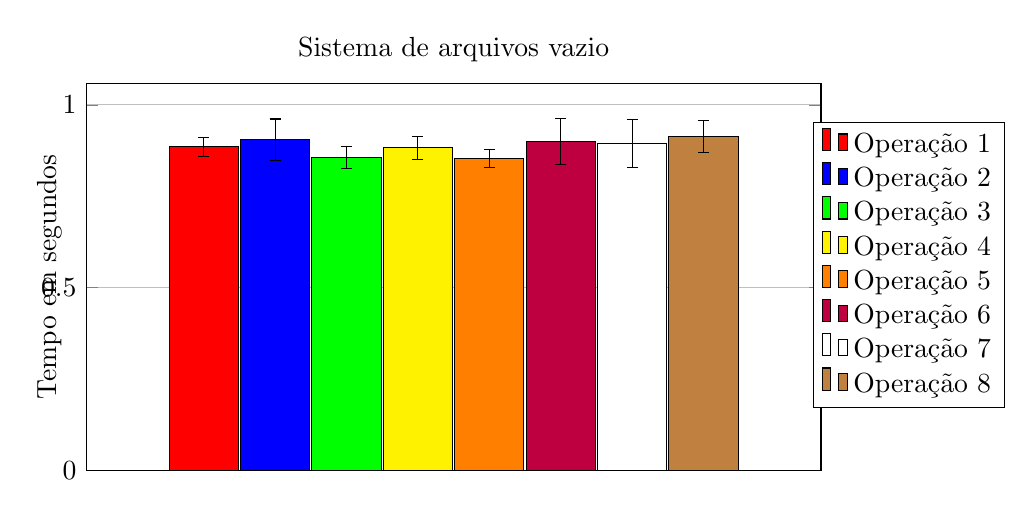
\begin{tikzpicture}
                \begin{axis}[
                        width  = 0.9*\textwidth,
                        height = 6.5cm,
                        major x tick style = transparent,
                        ybar=2*\pgflinewidth,
                        bar width=25pt,
                        ymajorgrids = true,
                        symbolic x coords={Sistema de arquivos vazio},
                        xtick = data,
                        xticklabel pos=right,
                        scaled y ticks = false,
                        enlarge x limits=0.50,
                        ymin=0,
                        ylabel={Tempo em segundos},
                        ylabel style={yshift=-0.5cm},
                        legend cell align=left,
                        % legend pos=north east,
                        legend style={at={(1.12,0.9)},anchor=north},
                    ]

                    \addplot[style={fill=red},
                    error bars/.cd,
                    y dir=both,
                    y explicit]
                    coordinates {
                        (Sistema de arquivos vazio, 0.8853333333333334) += (0,0.02595778558024465) -= (0,0.02595778558024465)
                    };

                    \addplot[style={fill=blue},
                    error bars/.cd,
                    y dir=both,
                    y explicit]
                    coordinates {
                        (Sistema de arquivos vazio, 0.9047999999999999) += (0,0.056439206590596584) -= (0,0.056439206590596584)
                    };

                    \addplot[style={fill=green},
                    error bars/.cd,
                    y dir=both,
                    y explicit]
                    coordinates {
                        (Sistema de arquivos vazio, 0.8555666666666668) += (0,0.03031087265297527) -= (0,0.03031087265297527)
                    };

                    \addplot[style={fill=yellow},
                    error bars/.cd,
                    y dir=both,
                    y explicit]
                    coordinates {
                        (Sistema de arquivos vazio, 0.8824333333333334) += (0,0.03186171263209405) -= (0,0.03186171263209405)
                    };

                    \addplot[style={fill=orange},
                    error bars/.cd,
                    y dir=both,
                    y explicit]
                    coordinates {
                        (Sistema de arquivos vazio, 0.8532) += (0,0.02341866214675493) -= (0,0.02341866214675493)
                    };

                    \addplot[style={fill=purple},
                    error bars/.cd,
                    y dir=both,
                    y explicit]
                    coordinates {
                        (Sistema de arquivos vazio, 0.8994666666666666) += (0,0.06373270507842371) -= (0,0.06373270507842371)
                    };

                    \addplot[style={fill=white},
                    error bars/.cd,
                    y dir=both,
                    y explicit]
                    coordinates {
                        (Sistema de arquivos vazio, 0.8942) += (0,0.06656332736164362) -= (0,0.06656332736164362)
                    };

                    \addplot[style={fill=brown},
                    error bars/.cd,
                    y dir=both,
                    y explicit]
                    coordinates {
                        (Sistema de arquivos vazio, 0.9133) += (0,0.04467808448400404) -= (0,0.04467808448400404)
                    };

                \legend{Operação 1, Operação 2, Operação 3, Operação 4, Operação
                5, Operação 6, Operação 7, Operação 8}
                \end{axis}
            \end{tikzpicture}
    \end{frame}
    \begin{frame}{Experimentos - Sistema de arquivos com \texttt{10MB} ocupado}
        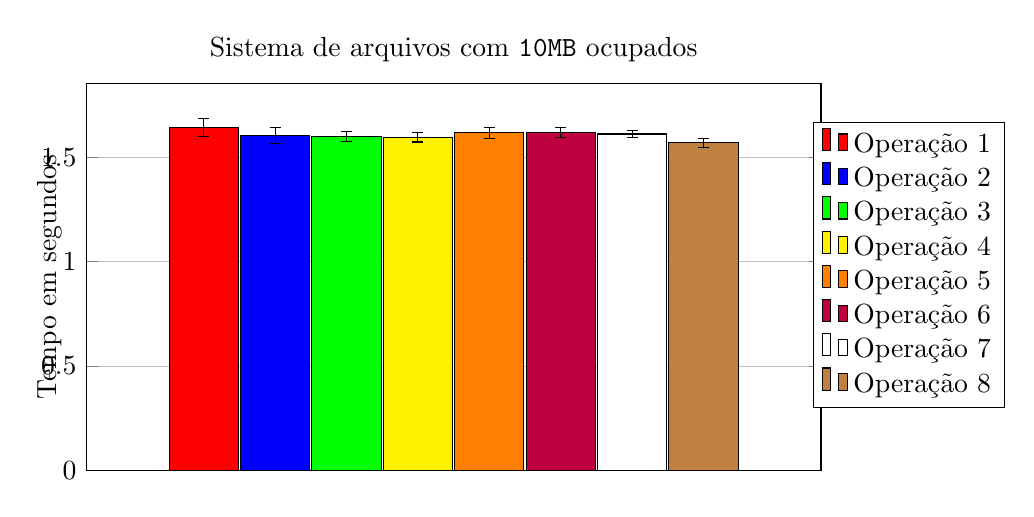
\begin{tikzpicture}
                \begin{axis}[
                        width  = 0.9*\textwidth,
                        height = 6.5cm,
                        major x tick style = transparent,
                        ybar=2*\pgflinewidth,
                        bar width=25pt,
                        ymajorgrids = true,
                        symbolic x coords={Sistema de arquivos com \texttt{10MB} ocupados},
                        xtick = data,
                        xticklabel pos=right,
                        scaled y ticks = false,
                        enlarge x limits=0.50,
                        ymin=0,
                        ylabel={Tempo em segundos},
                        ylabel style={yshift=-0.5cm},
                        legend cell align=left,
                        % legend pos=north east,
                        legend style={at={(1.12,0.9)},anchor=north},
                    ]

                    \addplot[style={fill=red},
                    error bars/.cd,
                    y dir=both,
                    y explicit]
                    coordinates {
                        (Sistema de arquivos com \texttt{10MB} ocupados, 1.6449333333333334) += (0,0.04293604361366569) -= (0,0.04293604361366569)
                    };

                    \addplot[style={fill=blue},
                    error bars/.cd,
                    y dir=both,
                    y explicit]
                    coordinates {
                        (Sistema de arquivos com \texttt{10MB} ocupados, 1.6056000000000004) += (0,0.037195424075949876) -= (0,0.037195424075949876)
                    };

                    \addplot[style={fill=green},
                    error bars/.cd,
                    y dir=both,
                    y explicit]
                    coordinates {
                        (Sistema de arquivos com \texttt{10MB} ocupados, 1.6001333333333332) += (0,0.023781569663101743) -= (0,0.023781569663101743)
                    };

                    \addplot[style={fill=yellow},
                    error bars/.cd,
                    y dir=both,
                    y explicit]
                    coordinates {
                        (Sistema de arquivos com \texttt{10MB} ocupados, 1.5977666666666663) += (0,0.023380707847622938) -= (0,0.023380707847622938)
                    };

                    \addplot[style={fill=orange},
                    error bars/.cd,
                    y dir=both,
                    y explicit]
                    coordinates {
                        (Sistema de arquivos com \texttt{10MB} ocupados, 1.6177333333333332) += (0,0.025500627947340575) -= (0,0.025500627947340575)
                    };

                    \addplot[style={fill=purple},
                    error bars/.cd,
                    y dir=both,
                    y explicit]
                    coordinates {
                        (Sistema de arquivos com \texttt{10MB} ocupados, 1.6184333333333336) += (0,0.02378984723037801) -= (0,0.02378984723037801)
                    };

                    \addplot[style={fill=white},
                    error bars/.cd,
                    y dir=both,
                    y explicit]
                    coordinates {
                        (Sistema de arquivos com \texttt{10MB} ocupados, 1.6125333333333332) += (0,0.017830096402122783) -= (0,0.017830096402122783)
                    };

                    \addplot[style={fill=brown},
                    error bars/.cd,
                    y dir=both,
                    y explicit]
                    coordinates {
                        (Sistema de arquivos com \texttt{10MB} ocupados, 1.5704999999999996) += (0,0.021161643961972024) -= (0,0.021161643961972024)
                    };

                \legend{Operação 1, Operação 2, Operação 3, Operação 4, Operação
                5, Operação 6, Operação 7, Operação 8}
                \end{axis}
            \end{tikzpicture}
    \end{frame}
    \begin{frame}{Experimentos - Sistema de arquivos com \texttt{50MB} ocupado}
        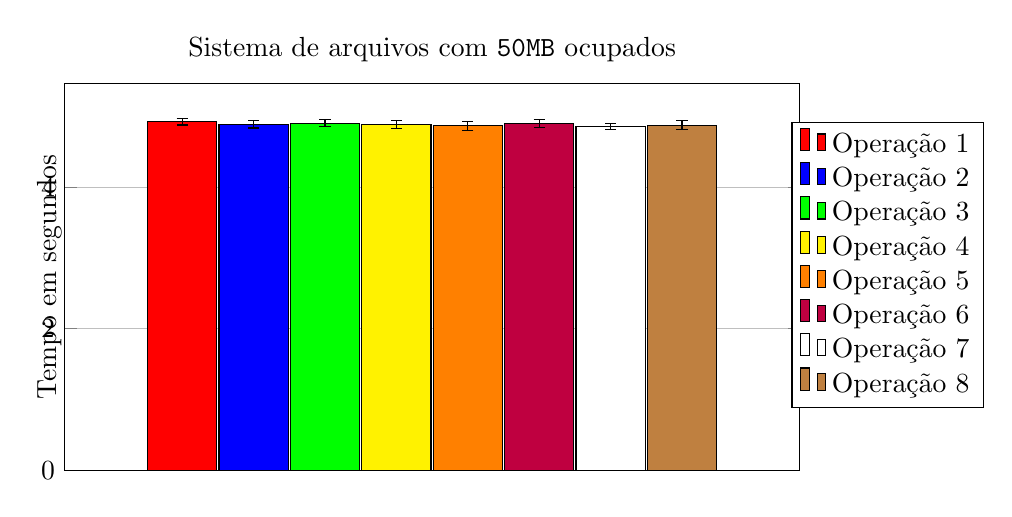
\begin{tikzpicture}
                \begin{axis}[
                        width  = 0.9*\textwidth,
                        height = 6.5cm,
                        major x tick style = transparent,
                        ybar=2*\pgflinewidth,
                        bar width=25pt,
                        ymajorgrids = true,
                        symbolic x coords={Sistema de arquivos com \texttt{50MB} ocupados},
                        xtick = data,
                        xticklabel pos=right,
                        scaled y ticks = false,
                        enlarge x limits=0.50,
                        ymin=0,
                        ylabel={Tempo em segundos},
                        ylabel style={yshift=-0.5cm},
                        legend cell align=left,
                        % legend pos=north east,
                        legend style={at={(1.12,0.9)},anchor=north},
                    ]

                    \addplot[style={fill=red},
                    error bars/.cd,
                    y dir=both,
                    y explicit]
                    coordinates {
                        (Sistema de arquivos com \texttt{50MB} ocupados, 4.9243999999999994) += (0,0.04773444251239711) -= (0,0.04773444251239711)
                    };

                    \addplot[style={fill=blue},
                    error bars/.cd,
                    y dir=both,
                    y explicit]
                    coordinates {
                        (Sistema de arquivos com \texttt{50MB} ocupados, 4.886500000000001) += (0,0.05134719477640183) -= (0,0.05134719477640183)
                    };

                    \addplot[style={fill=green},
                    error bars/.cd,
                    y dir=both,
                    y explicit]
                    coordinates {
                        (Sistema de arquivos com \texttt{50MB} ocupados, 4.902833333333333) += (0,0.04610089843517922) -= (0,0.04610089843517922)
                    };

                    \addplot[style={fill=yellow},
                    error bars/.cd,
                    y dir=both,
                    y explicit]
                    coordinates {
                        (Sistema de arquivos com \texttt{50MB} ocupados, 4.888266666666666) += (0,0.05815751200847479) -= (0,0.05815751200847479)
                    };

                    \addplot[style={fill=orange},
                    error bars/.cd,
                    y dir=both,
                    y explicit]
                    coordinates {
                        (Sistema de arquivos com \texttt{50MB} ocupados, 4.866666666666665) += (0,0.06325911258107837) -= (0,0.06325911258107837)
                    };

                    \addplot[style={fill=purple},
                    error bars/.cd,
                    y dir=both,
                    y explicit]
                    coordinates {
                        (Sistema de arquivos com \texttt{50MB} ocupados, 4.8954666666666675) += (0,0.05888239409881237) -= (0,0.05888239409881237)
                    };

                    \addplot[style={fill=white},
                    error bars/.cd,
                    y dir=both,
                    y explicit]
                    coordinates {
                        (Sistema de arquivos com \texttt{50MB} ocupados, 4.8537333333333335) += (0,0.04546235865175731) -= (0,0.04546235865175731)
                    };

                    \addplot[style={fill=brown},
                    error bars/.cd,
                    y dir=both,
                    y explicit]
                    coordinates {
                        (Sistema de arquivos com \texttt{50MB} ocupados, 4.875166666666667) += (0,0.06050618529693447) -= (0,0.06050618529693447)
                    };

                \legend{Operação 1, Operação 2, Operação 3, Operação 4, Operação
                5, Operação 6, Operação 7, Operação 8}
                \end{axis}
            \end{tikzpicture}
    \end{frame}

    \begin{frame}{Experimentos - Especificações do hardware e SO}
        \begin{itemize}
            \justifying
            \item Os testes foram executados em um Ubuntu 20.10 com versão do
                kernel 5.8.0-31-generic e sistema de arquivos EXT4 com
                journaling.
            \item O SO em questão se encontra dentro de uma máquina virtual
            \item O hardware utilizado foi:
                \begin{itemize}
                    \justifying
                    \item processador Intel i7 7700 3.6GHz com 4 cores dedicados
                        para a VM
                    \item memória 12Gb de memória RAM 2400MHz dedicados para a
                        VM
                    \item disco HD WD SATA 7200RPM 6,0Gb/s
                \end{itemize}
        \end{itemize}
    \end{frame}

    \begin{frame}{Conclusões - Tempo}
        \begin{itemize}
            \justifying
            \item É possível observar que o tempo de execução das operações em
                um mesmo sistema de arquivos levam uma quantidade de tempo
                similar;
            \item Isso se deve ao fato de que na nossa implementação, precisamos
                dar \texttt{umount} para salvar as alterações de um comando no
                disco. Assim sendo, em todos nossos testes, além dos comandos
                pedidos, também executamos \texttt{mount}, \texttt{umount} e
                \texttt{sai};
            \item O tempo de execução foi, portanto, dominado por esses comandos
                e vemos que existe pouca diferença entre o tempo de execução de
                cada operação (mesmo quando removemos vários subdiretórios e
                arquivos no teste 8);
        \end{itemize}

    \end{frame}

    \begin{frame}{conclusões - Tempo}
        \begin{itemize}
            \justifying
            \item Além disso, podemos observar que o tempo gasto por teste aumenta
                linearmente com a quantidade de bytes ocupados (mesmo
                mantendo \texttt{100MB} fixos para o disco).
        \end{itemize}
    \end{frame}

    \begin{frame}
        \centering
        {\huge Obrigado!}

        $ \\ $

        Lucas e Marcos

    \end{frame}
\end{document}
